\begin{figure}[t]
  \centering
  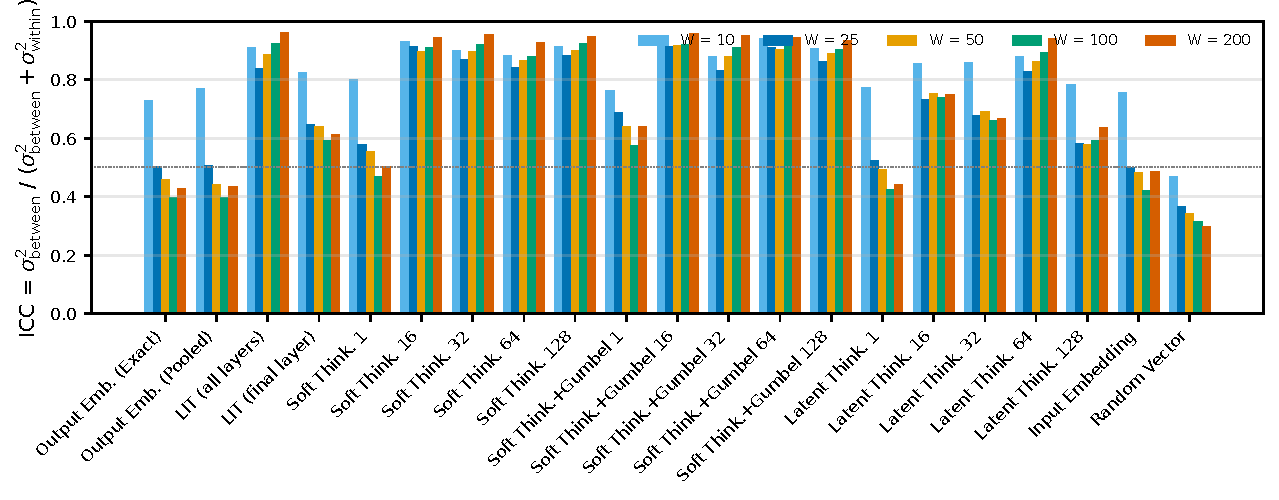
\includegraphics[width=\linewidth]{figures/pdf/causality_kl_variance_70b.pdf}
  \caption{Intraclass correlation $\mathrm{ICC} = \sigma^2_{\text{between}} / (\sigma^2_{\text{between}} + \sigma^2_{\text{within}})$ of per-beam causality KL on Llama-3.3-70B, with bars per averaging window. Values above $0.5$ indicate that the per-problem mean carries most of the dispersion, validating the cluster bootstrap that resamples problems and keeps within-problem beams glued together (\cref{appendix:sub:bootstrap}).}
  \label{fig:causality-kl-variance}
\end{figure}
